\documentclass[../main.tex]{subfiles}
\begin{document}

\subsection{Global-best guided Quantum-inspired Tabu Search Algorithm with Not-gate (GNQTS)}
\textbf{What is GNQTS and its evolution}

\textbf{Flow chart of GNQTS}

\begin{figure}
    \centering
    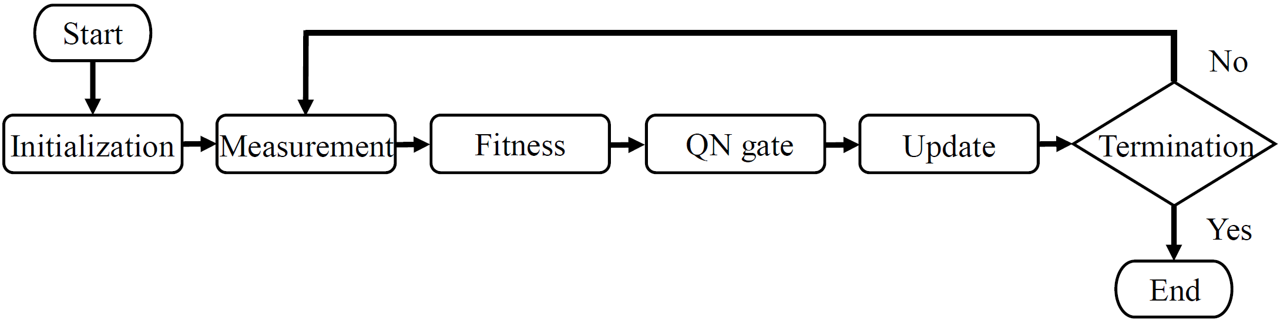
\includegraphics[scale = 0.5] {figure/flowChart.png}
    \captionsetup{font={footnotesize}}
    % \vspace{-3em}
    \caption{The flowchart of GNQTS}
    % \vspace{-0.5em}
    \label{flow}
\end{figure}

\textbf{Pseudo code of GNQTS}

\begin{algorithm}
    \caption{GNQTS}
    \begin{algorithmic}[1]
        \State $i \leftarrow 0$
        \State Initialize quantum  population $Q(0)$
        \State Initialize best solution $b$
        \While {not termination-condition}
        \State {$i \leftarrow i + 1$}
        \State Produce neighborhood set N by measure $Q(i-1)$
        \State Evaluate $f(s)$
        \State Find the best solution $s^b$ and the worst solution $s^w$
        \State Update $b$
        \State Detect whether GNQTS is stuck in local optimal
        \If {stuck}
        \State Do Quantum Not Gate
        \EndIf
        \State Update $Q(i)$
        \EndWhile
    \end{algorithmic}
\end{algorithm}
\bigbreak
\textbf{Explain each step of GNQTS}

\subsection{Sliding Windows}
\textbf{What are sliding windows}

\textbf{Old sliding sindows}

\textbf{New sliding windows}

\textbf{What can new sliding windows achieve}

\subsection{Technical Indicators}
% \textbf{What are technical indicators}

Technical indicators are the rule of thumb or pattern-based signals produced mathematically by the stock price or volume. The fundatioin of technical indicators is the historical prices of the stocks. It is belived that the history will repeated itself as the time extends. In other words, patterns of the market behavior continously appears throughout the history of the stock market. By analyzing the historical data, technical analysis use indicators to determine the timing to buy or sell stocks.

\subsubsection{Simple Moving Average (SMA)}

% \textbf{What is Simple Moving Average}
A Moving Average is an indicator that shows the trend of stock price of a company. If the moving average was decreasing, it indecates that the price is falling recently. If the moving average was increasing, it indecates that the price is rising recently. There are several different types of moving averages. The most polpular one is the simple moving average (SMA). The major difference between moving averages is the weight applies to the stock price when calculating the indecator.
\bigbreak

% \textbf{SMA formula}
SMA is a indicator which can be easily calculated compare to the other moving averages because the weight that applies to stocks price when calculate SMA is equally weighted. SMA is the average closed price of a certain period of time (e.g., 5 days). The period of days that is been used to calculate the averge price is called look-back period. The formula of SMA is shown in \ref{SMA}, where $n$ is the look-back period and $t$ is the date of today.

\begin{equation}\label{SMA}\scalebox{1}
    {$SMA_{n} = \dfrac{price_{t-n}+price_{t-n+1}+price_{t-n+2}+...+price_{t-2}+price_{t-1}}{n}$}
\end{equation}
\bigbreak

% \textbf{How to use SMA}
The most common method of using SMA is to compare the relationship between two trends of SMA, which is called crossover. The way to define a crossover is that when plotting two different SMA values, the line of the first SMA passes through the line of the second SMA from below. This is also called a golden crossover. On the other hand, a death crossover is that when the line of first SMA passes through the line of second SMA from above. We can simplify the trading strategy of using these two SMA into SMA($1_{st}$ SMA, $2_{nd}$ SMA). Figure \ref{cross_demo} demostrate the timimg of golden cross and death cross when using SMA(5, 20). These two types of crossover are the important signal of determining the timing of buying or selling the stocks. A buy signal is triggered when a golden cross appears. A selling signal is triggered when a death cross appears.
\bigbreak

\begin{figure}
    \centering
    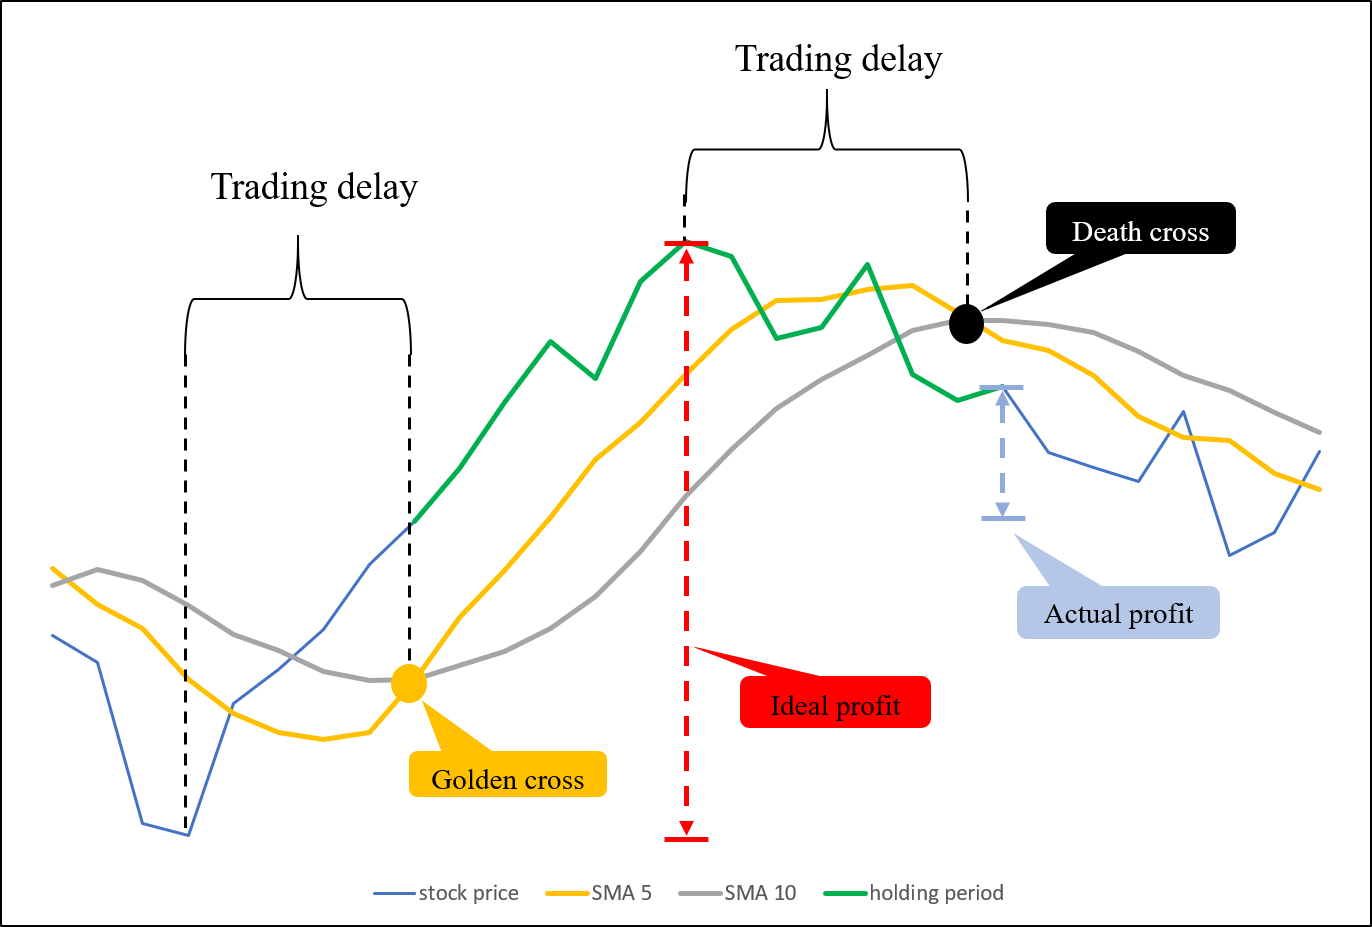
\includegraphics[scale = 0.6] {figure/cross1.png}
    \captionsetup{font={footnotesize}}
    % \vspace{-3em}
    \caption{Demostration of using strategy SMA(5, 20)}
    % \vspace{-0.5em}
    \label{cross_demo}
\end{figure}

% \textbf{Characteristics of SMA}

\bigbreak

\subsubsection{Relative Strength Index (RSI)}
\textbf{What is RSI}

\textbf{How to use RSI}

\textbf{Characteristics of RSI}

\textbf{RSI formula}

Relative Strength Index (RSI) was developed by J. Welles Wilder, Jr. [3] in 1978. This index is a widely used technical indicator of the financial market for measuring the magnitude of recent price changes. RSI regards a rising stock price as strength from buyers, a falling price as strength from sellers, and the closing price is the outcome of the relative strength of buyers and sellers. Here are the formulae for calculating RSI. The calculating process can be divided into two steps. For step one (as shown in formulae \ref{step_1}), the average gain and loss is the average of rice and drop respectively during the look-back period. As for step two, with the RSI in step one, we can recursively calculate the next RSI using formula 2, where $N$ is a parameter, representing a look-back period. The formulae for calculating RSI are as follows.

\begin{equation}\label{step_1}\scalebox{1}
    {$RSI_{step\ one}=100-\left[\dfrac{100}{1+\dfrac{Average\ gain}{Average\ loss}}\right]$}
    \vspace{1em}
\end{equation}

\begin{equation}\label{step_2}\scalebox{1}
    {$RSI_{step\ two}=100-\left[\dfrac{100}{1+\dfrac{Previous\ Average\ Gain\times(N-1)+Current\ Gain}{-(Previous\ Average\ Loss)\times(N-1)+Current\ Loss}}\right]$}
    \vspace{1em}
\end{equation}

\subsection{Normalize Internal Rate of Return}
How to evaluate the performance of our method

% \subsection{Investment Targets}
% what are DJI 30s

% what is DJI

% what is IXIC

% what is NYA

% Why choose these investment targets


\end{document}